\Subsection{Ряды в нормированных пространствах}
%BEGIN TICKET 54
\begin{definition}
    $X$ --- пространство с нормой,  $x_n \in X$.

     $\sum\limits_{k=1}^\infty x_k$ --- ряд. Частичная сумма ряда  $S_n \coloneqq \sum\limits_{k=1}^n x_k$.

     Если  $\exists \lim\limits_{n \to \infty}$, то он называется суммой ряда.

     Ряд сходится, если у него есть сумма (и для $\R$ эта сумма конечна), иначе она бесконечна.
\end{definition}
\begin{theorem}[Необходимое условие сходимости]
    Если ряд $\sum\limits_{n=1}^\infty x_k$ --- сходится, то  $\lim x_n = 0$.
\end{theorem}
\begin{proof}
    $S_n \coloneqq \sum\limits_{k=1}^n x_k \to S \implies \underbrace{S_n - S_{n-1}}_{x_n} \to S - S = 0$.
\end{proof}
\begin{properties}
    \begin{enumerate}
        \item Линейность. $\sum\limits_{n=1}^\infty (\alpha x_n + \beta y_n) = \alpha \sum\limits_{n=1}^\infty x_n + \beta \sum\limits_{n=1}^\infty y_n$.
        \item Расстановка скобок. В ряду произвольным образом можно ставить скобки, расстановка скобок дает тот же результат. 

            \textbf{Набросок доказательства:} мы просто смотрим на предел подпоследовательности.
        \item В  $\CC$ и  $\R^n$ сходимость равносильна покоординатной сходимости.
    \end{enumerate}
\end{properties}
\begin{theorem}[Критерий Коши]
    $X$ --- полное нормированное пространство.

    Тогда ряд  $\sum\limits_{n=1}^\infty x_n$ сходится  $\iff \forall \eps > 0 \exists N \forall m,n \ge N\!: \| \sum\limits_{k=m}^n x_k \| < \eps$.
\end{theorem}
\begin{proof}
    $S_n \coloneqq \sum\limits_{k=1}^n x_k$. Последовательность  $S_n$ сходится  $\iff S_n$ --- фундаментальная  $\iff \forall \eps > 0 \exists N \forall m, n > N\!: \|S_n-S_m\| < \eps \iff \| \sum\limits_{k=m+1}^n x_k \| < \eps$.
\end{proof}
%END TICKET 54
%BEGIN TICKET 55
\begin{definition}
    Ряд $\sum\limits_{n=1}^\infty x_n$ сходится абсолютно, если  $\sum\limits_{n=1}^\infty \|x_n\|$ сходится.
\end{definition}
\begin{remark}
    В частности, в $\R$ абсолютная сходимость --- сходимость ряда  $\sum\limits_{n=1}^\infty |x_n|$.
\end{remark}
\begin{theorem}
    $X$ --- полное нормированное пространство.

    Если  $\sum\limits_{n=1}^\infty x_n$ абсолютно сходится, то он сходится.
\end{theorem}
\begin{proof}
    Пусть $\sum\limits_{n=1}^\infty \|x_n\|$ --- сходится. Тогда  $\forall \eps > 0 \exists N \forall m, n \ge N\!: \sum\limits_{k=m+1}^n \|x_k\| < \eps$. Воспользуемся свойством о том, что сумма норм не меньше, чем норма суммы. А значит получили $\forall \eps > 0 \exists N \forall m, n \ge N\!: \| \sum\limits_{k=m+1}^n x_k\| < \eps$, что является критерием Коши для исходной последовательности.
\end{proof}
\begin{theorem}
    \begin{enumerate}
        \item $X$ --- нормированное пространство. Если  $\lim x_n = 0$ и в каждой скобке  $\le M$ слагаемых то из сходимости ряда после расстановки скобок следует сходимость исходнного
        \item $\R$. Если в каждой скобке все члены одного знака, то из сходимости ряда после расстановки скобок следует сходимость исходного.
    \end{enumerate}
\end{theorem}
\begin{proof}
    $S_n \coloneqq \sum\limits_{k=1}^n x_k$ и  $S_{n_k} \to S$.
     \begin{enumerate}
         \item Возьмем $n$:  $n_k \le n < n_{k+1}$. $S_n = S_{n_k} + x_{n_k} + x_{n_k + 1} + x_{n_k  + 2} + \ldots + x_n$. $\|S_n - S\| \le \|S_{n_k} - S\| + \|x_{n_k + 1}\| + \ldots + \|x_n\|$. Мы знаем, что $S_{n_k} \to S \implies \exists K \forall k \ge K\!: \|S_{n_k} - S\| < \eps$.

             $\lim x_j = 0 \implies \exists J \forall j \ge J \|x_j\| < \eps$. Следовательно исходная сумма не более $(M+1)\eps$.
         \item  $n_k \le n < n_{k+1}$. Пусть в этом блоке неотрицательные слагаемые. $S_n = S_{n_k} + x_{n_k + 1} + x_{n_k + 2} + \ldots + x_n \ge S_{n_k}$. А еще знаем, что $S_n = S_{n_{k+1}} - x_{n_{k+1}} - x_{n_{k+1} - 1} - \ldots - x_{n+1} \le S_{n_{k+1}}$. Откуда получаем, что $S_{n_k} \le S_n \le S_{n_{k+1}}$, где всё $\to S$.
    \end{enumerate}
\end{proof}
%END TICKET 55
\Subsection{Знакопостоянные ряды}
%BEGIN TICKET 56
\begin{theorem}
    Пусть $a_n \ge 0$.

    Тогда сходимость ряда $\sum\limits_{n=1}^\infty a_n$ равносильная ограниченности последовательности  $S_n = \sum\limits_{k=1}^n a_k$.
\end{theorem}
\begin{proof}
    $S_1 \le S_2 \le \ldots$. Монотонная возрастающая последовательность имеет предел $\iff$ она ограничена.
\end{proof}
\begin{theorem}[Признак сравнения]
    Пусть $0 \le a_n \le b_n$. Тогда 
    \begin{enumerate}
        \item Если $\sum\limits_{n=1}^\infty b_n$ сходится, то  $\sum\limits_{n=1}^\infty a_n$ --- сходится.
        \item  Если $\sum\limits_{n=1}^\infty a_n$ --- расходится, то $\sum\limits_{n=1}^\infty b_n$ расходится.
    \end{enumerate}
\end{theorem}
\begin{proof}
    \begin{enumerate}
        \item $A_n \coloneqq \sum\limits_{k=1}^n a_k \le \sum\limits_{k=1}^n b_k = B_n$.

            $\sum b_n$ --- сходится  $\implies B_n$ --- ограничена  $\implies A_n$ ограничена  $\implies \sum a_n$ сходится.
        \item Отрицание 1.
    \end{enumerate}
\end{proof}
\begin{consequence}
    \begin{enumerate}    
        \item Пусть $a_n, b_n \ge 0$. Если $a_n = \mathcal{O}(b_n)$ и  $\sum\limits_{n=1}^\infty b_n$ --- сходится, то  $\sum\limits_{n=1}^\infty a_n$ --- сходится.
        \item Пусть $a_n, b_n \ge 0$, Если $a_n \sim b_n$, то ряды ведут себя одинаково.
    \end{enumerate}
\end{consequence}
\begin{proof}
    \begin{enumerate}
        \item $a_n = \mathcal{O}(b_n) \implies 0 \le a_n \le Cb_n$. $\sum\limits_{n=1}^\infty Cb_n = C \sum\limits_{n=1}^\infty b_n$ --- сходится  $\implies \sum a_n$ --- сходится.
        \item $a_n = b_nc_n$, где  $\lim c_n = 1 \implies \frac{1}{2} \le c_n \le 2$ при $n\ge N$. Тогда $a_n = \mathcal{O}(b_n)$ и  $b_n = \mathcal{O}(a_n)$.
    \end{enumerate}
\end{proof}
%END TICKET 56
%BEGIN TICKET 57
\begin{theorem}[Признак Коши]
    Пусть $a_n \ge 0$.
    \begin{enumerate}
        \item Если $\sqrt[n]{a_n} \le q < 1$, то ряд сходится.
        \item $\sqrt[n]{a_n} > 1$, то ряд расходится.
        \item  Пусть $\varlimsup \sqrt[n]{a_n} \eqqcolon q^*$. Если  $q^* > 1$, то ряд расходится, если  $q^* < 1$, то ряд сходится.
    \end{enumerate}
\end{theorem}
\begin{remark}
    Если $q^* = 1$, то ряд может сходиться, а может расходиться.  $\sum\limits_{n=1}^\infty \frac{1}{n(n+1)}$ --- сходится, $\sqrt[n]{\frac{1}{n(n+1)}} \to 1$.

    $\sum\limits_{n=1}^\infty \frac{1}{n}$ --- расходится. $\sqrt[n]{a_n} = \frac{1}{\sqrt[n]{n}} \to 1$.
\end{remark}
\begin{proof}
    \begin{enumerate}
        \item $\sqrt[n]{a_n} \le q < 1 \implies a_n \le q^n$. По признаку сравнения с геометрической прогрессией $\sum\limits_{n=1}^\infty q^n$ --- сходится.
        \item  $\sqrt[n]{a_n} \ge 1 \implies a_n \centernot \to 0 \implies $ расходится.
        \item Если $q^* > 1$. Найдется  $n_k\!: \sqrt[n_k]{a_{n_k}} \to q^*  > 1$ (по определению верхнего предела)  $\implies$ начиная с некоторого номера $\sqrt[n_k]{a_{n_k}} > 1 \implies a_{n_k} > 1 \implies a_n \centernot \to 0$ и ряд расходится.

            Если $q^* < 1$,  $q^* = \lim\limits_{n \to \infty} \sup\limits_{k \ge n} \sqrt[k]{a_k} \implies$ для больших $n$  $\sup_{k \ge n} \sqrt[k]{a_k} < q < 1$. Но при этом $\sqrt[n]{a_n} \le \sup\limits_{k \ge n}\sqrt[k]{a_k}$, а значит $\sqrt[n]{a_n} < q$ при больших  $n \implies$ ряд сходится.
    \end{enumerate}
\end{proof}
%END TICKET 57
%BEGIN TICKET 58
\begin{theorem}[Признак Даламбера]
    Пусть $a_n > 0$. Тогда
     \begin{enumerate}
         \item $\frac{a_{n+1}}{a_n} \le d < 1$, то ряд сходится.
         \item Если  $\frac{a_{n+1}}{a_n} \ge 1$, то ряд расходится.
         \item Пусть  $\lim \frac{a_{n+1}}{a_n} = d^*$. Если $d^* < 1$, то ряд сходится. Если  $d^* > 1$, то ряд расходится.
    \end{enumerate}
\end{theorem}
\begin{remark}
    С единицей все еще ничего непонятно. Смотри предыдущие примеры.
\end{remark}
\begin{proof}
    \begin{enumerate}
        \item $\frac{a_n}{a_1} = \frac{a_n}{a_{n-1}} \cdot \frac{a_{n-1}}{a_{n-2}} \cdot \ldots \cdot \frac{a_2}{a_1} \le d^{n-1}$. $a_n \le d^{n-1} \cdot a_1$ и ряд мажорируется геометрической прогрессией $\sum\limits_{n=1}^\infty a_1 \cdot d^{n-1}$. Она сходится $\implies \sum\limits_{n=1}^\infty a_n$ --- сходится.
        \item $a_{n+1} \ge a_n \implies a_n \ge a_1 > 0$ и $a_n \centernot \to 0 \implies$ ряд расходится. 
        \item Еcли  $d^* > 1$. Тогда  $\frac{a_{n+1}}{a_n} \ge 1$ при $n \ge N \implies a_n \ge a_N > 0 \quad \forall n \ge N \implies a_n \centernot \to 0$ и ряд расходится.

            Если $d^* < 1$. Так как  $\lim \frac{a_{n+1}}{a_n} = d^* \implies \frac{a_{n+1}}{a_n} < d$ при $n \ge N \implies$ ряд сходится по признаку 1.
    \end{enumerate}
\end{proof}
\begin{example}
    $\sum\limits_{n=0}^\infty \frac{x^n}{n!}$.

    Даламбер. $\frac{a_{n+1}}{a_n} = \frac{x^{n+1}}{(n+1)!} : \frac{x^n}{n!} = \frac{x}{n+1} \to 0 < 1$. Ряд сходится.

    Коши. $\sqrt[n]{a_n} = \sqrt[n]{\frac{x^n}{n!}} = \frac{x}{\sqrt[n]{n!}} \sim \frac{x}{\sqrt[n]{n^ne^{-n}\sqrt{2\pi n}}} = \frac{x}{n e^{-1}\sqrt[2n]{2\pi n}} \sim \frac{xe}{n} \to 0$.
\end{example}
\begin{theorem}
    Пусть $a_n > 0$ и  $\lim\limits_{n \to \infty} \frac{a_{n+1}}{a_n} = d^*$. Тогда $\lim \sqrt[n]{a_n} = d^*$.
\end{theorem}
\begin{proof}
    $\lim \frac{a_{n+1}}{a_n} = d^* \implies \lim \frac{\ln a_{n+1} - \ln a_n}{(n+1) - n} = \ln d^* \xRightarrow{\text{т. Штольца}} \lim \frac{\ln a_n}{n} = \ln d^* \implies \lim \sqrt[n]{a_n} = d^*$.
\end{proof}
%END TICKET 58
%BEGIN TICKET 59
\begin{theorem}
    Пусть $f$ неотрицательная монотонная  $\!: [1, +\infty) \to \R$. Тогда:
     \[
    \left| \sum_{k=a}^b f(k) - \int\limits_a^b f(x)\mathrm{d}x \right| \le \max\{f(a), f(b)\} 
    .\] 
\end{theorem}
\begin{proof}
     $\sum\limits_{k=a}^{b-1} f(k) \ge \int\limits_a^b f(x)\mathrm{d}x \ge \sum\limits_{k=a+1}^b f(k)$. Не поняли? Рисуем картинку!
     \begin{figure}[!h]
         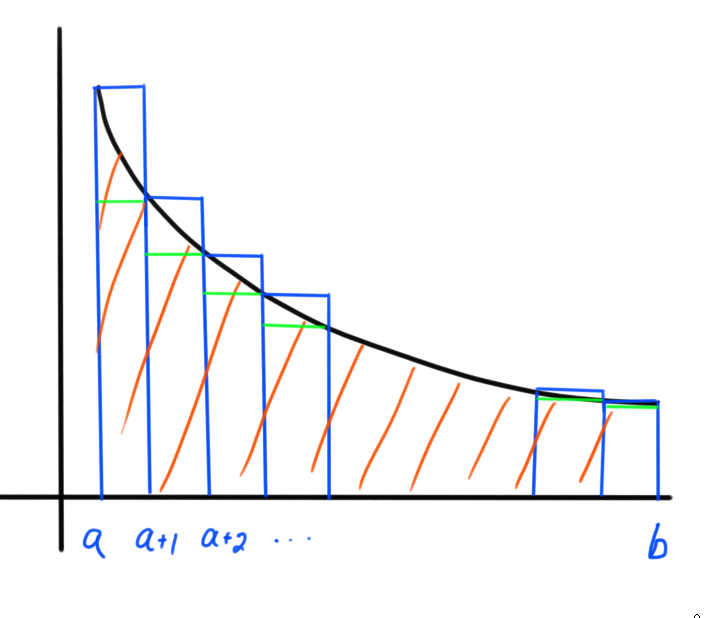
\includegraphics[scale=0.3]{integrals_and_sums}
     \end{figure}
    
    $\sum\limits_{k=a}^b f(k) - \int\limits_a^b \le \sum\limits_{k=a}^b - \sum\limits_{k=a-1}^b = f(a)$ (аналогично $f(b) = \sum\limits_{k=a}^b - \sum\limits_{k=a}^{b-1}$)

\end{proof}
\begin{theorem}[интегральный признак сходимости ряда]
    Пусть $f\!:[1, +\infty) \to \R$ неотрицательная, монотонно убывающая. 

    Тогда  $\sum\limits_{n=1}^\infty f(n)$ и  $\int\limits_1^\infty f(x) \mathrm{d}x$ ведут себя одинаково.
\end{theorem}
\begin{proof}
    По предыдущей теореме $S_n \coloneqq \sum\limits_{k=1}^n f(k) \ge \int\limits_1^n f(x)\mathrm{d}x \ge \sum\limits_{k=2}^n f(k) = S_n - f(1)$.

    Если ряд сходится, то $S_n$ --- ограничена  $\implies \int\limits_1^n f(x)\mathrm{d}x$ ограничена $\implies F(x) = \int\limits_1^x f$ --- ограничена $\implies \int\limits_1^\infty f(x)$ сходится.

    Если  $\int$ сходится $\implies \int\limits_1^n f$ --- ограничена  $\implies S_n$ --- ограничена  $\implies$ ряд сходится.
\end{proof}
\begin{example}
     \begin{enumerate}
         \item $\sum\limits_{n=1}^\infty \frac{1}{n^p}$, $p > 0$ (иначе члены ряда $\centernot \to 0$ и ряд расходится).\\
             $f(x) = \frac{1}{x^p}$. Монотонно убывает. $\sum \frac{1}{n^p}$ и $\int\limits_1^\infty \frac{\mathrm{d}x}{x^p}$ ведут себя одинаково: сходятся при  $p > 1$.
         \item $\sum\limits_{n=2}^\infty \frac{1}{n\ln n}$. $f(x) = \frac{1}{x\ln x}$ монотонно убывает. Поэтому $\int\limits_2^\infty \frac{\mathrm{d}x}{x\ln x}$ и $\sum\limits_{n=2}^\infty \frac{1}{n \ln n}$ ведут себя одинаково. 

             Там можно посчитать интеграл (разойдется).
    \end{enumerate}
\end{example}
\begin{consequence}
    \begin{enumerate}
        \item Если $a_n > 0$ и  $a_n = \mathcal{O}(\frac{1}{n^p})$ при $p > 1$ --- ряд  $\sum a_n$ --- сходится.
        \item Если  $a_n > 0$ и  $a_n \sim \frac{c}{n^p}$, то при $p > 1$ ряд  $\sum a_n$ --- сходится, а иначе расходится.
    \end{enumerate}
\end{consequence}
%END TICKET 59

\Subsection{Знакопеременные ряды}
\begin{definition}
    $\sum a_n$ --- сходится, но не абсолютно  $=$ ряд сходится условно.
\end{definition}
\begin{theorem}[Преобразование Абеля]
    $\sum\limits_{k=1}^n a_n b_n$.  $A_k \coloneqq a_1 + a_2 + \ldots + a_k$. Хочется заменить $a_n \to A_n$.

    Формулу сложнее запомнить, чем вывести, поэтому сначала выпишем её.
\end{theorem}
\begin{proof}
    \begin{align*}
        \sum_{k=1}^n a_k b_k &= \sum_{k=1}^n (A_k - A_{k-1})b_k = \sum_{k=1}^n A_kb_k - \sum_{j=2}^n A_{j-1}b_j \overset{k=j-1}{=} \sum_{k=1}^n A_kb_k - \sum_{k=1}^{n-1}A_kb_{k+1}  = \\ &= A_nb_n + \sum_{k=1}^{n-1}A_k(b_k - b_{k+1}).
    \end{align*}
\end{proof}
\begin{theorem}[Признак Дирихле]
    \begin{enumerate}
        \item $A_n$ (частичные суммы) --- ограничены ($|A_n| \le M$),
        \item $b_n$ монотонны,
        \item  $b_n \to 0$.
    \end{enumerate}
    Тогда $\sum\limits_{n=1}^\infty a_nb_n$ --- сходится.
\end{theorem}
\begin{proof}
    \begin{align*}
    S_n \coloneqq \sum_{k=1}^n a_k b_k = \underbracket{A_nb_n}_{\mathclap{\text{огр. на б.м.}}} + \sum\limits_{k=1}^{n-1}A_k(b_k-b_{k+1})
    \end{align*}
    Надо показать, что $\sum\limits_{k=1}^\infty A_k(b_k - b_{k+1})$ --- сходится. Для этого докажем, что ряд абсолютно сходится: $\sum\limits_{k=1}^\infty |A_k||b_k - b_{k+1}|$ --- сходится. 

    Мы знаем, что $\sum\limits_{k=1}^\infty |A_k||b_k - b_{k+1}| \le \sum\limits_{k=1}^\infty M \cdot |b_k - b_{k+1}| \overset{(*)}{=} M|\sum\limits_{k=1}^\infty (b_k - b_{k+1})| \le M|b_1|$.

    $(*)$ --- у нас постоянная монотонность, следовательно все слагаемые одного знака.
\end{proof}
\begin{theorem}[Признак Абеля]
    \begin{enumerate}
        \item Ряд $\sum\limits_{n=1}^\infty a_n$ --- сходится,
        \item $b_n$ --- монотонны,
        \item $b_n$ --- ограничены.
    \end{enumerate}
    Следовательно, $\sum\limits_{n=1}^\infty a_nb_n$ сходится.
\end{theorem}
\begin{proof}
    $2) + 3) \implies \exists \R \ni b \coloneqq \lim b_n$. Тогда  $\widetilde{b}_n \coloneqq b_n - b$ монотонны и  $\to 0$.

     $\sum\limits_{n=1}^\infty a_n$ --- сходится  $\implies A_n$ имеет предел  $\implies$  $A_n$ --- ограничены.

     Тогда  $\sum\limits_{n=1}^\infty a_n \widetilde{b}_n$ --- сходится  по признаку Дирихле. $\sum\limits_{n=1}^\infty a_n \widetilde{b}_n = \sum\limits_{n=1}^\infty a_n(b_n - b) \implies \sum\limits_{n=1}^\infty a_n b_n = b\underbracket{\sum\limits_{n=1}^\infty a_n}_{\mathclap{\text{по усл.}}} + \underbracket{\sum\limits_{n=1}^\infty a_n \widetilde{b}_n}_{\mathclap{\text{выяснили}}}$. 
\end{proof}
\begin{example}
    $\sum\limits_{n=1}^\infty \frac{\sin n)}{n^p}$ - сходится при $p > 0: a_n = \sin n, b_n = \frac{1}{n^p}, |A_n| \leq 2$.
\end{example}
\begin{example}
    $\sum\limits_{n=1}^\infty \frac{1}{n^3 \sin^2 n}$ - сходимость неизвестна.
\end{example}
\begin{definition}
    Знакочередующийся ряд $\sum\limits_{n=1}^\infty (-1)^{n-1}a_n$,  $a_n \ge 0$.
\end{definition}
\begin{theorem}[Признак Лейбница]
    Пусть есть ряд $\sum\limits_{n=1}^\infty (-1)^{n-1} a_n$.  $a_n \ge 0$ и монотонно стремится к 0.

    Тогда ряд $\sum\limits_{n=1}^\infty (-1)^{n-1} a_n$ сходится (по Дирихле: $a_n = (-1)^{n-1}, b_n = a_n$). Более того,  $S_{2n} \le S \le S_{2n+1}$.
\end{theorem}
\begin{proof}
    $S_{2n+2} = S_{2n} + a_{2n +1} - a_{2n+2} \ge S_{2n}$. $S_{2n+3} = S_{2n+1} - a_{2n+2} + a_{2n+3} \le S_{2n+1}$.

    $[0, S_1] \supset [S_2, S_3] \supset [S_4, S_5] \supset \ldots \supset [S_{2n}, S_{2n+1}] \supset \ldots$. $S_{2n+1} - S_{2n} = a_{2n+1} \to 0$.

    Пусть  $S$ их общая точка. Тогда  $\lim S_{2n} = \lim S_{2n+1} = S$.
\end{proof}

\begin{example}[Ряд Лейбница]
    \[
           \sum\limits_{n=1}^\infty \frac{(-1)^{n-1}}{n}
    .\] 
   \begin{align*}
       S_{2n}&=1-\frac{1}{2} + \frac{1}{3} - \frac{1}{4} + \ldots + \frac{1}{2n-1} - \frac{1}{2n} = H_{2n} - 2(\frac{1}{2} + \frac{1}{4} + \ldots + \frac{1}{2n}) = H_{2n} - H_n = \\ 
          &= \ln 2n+ \gamma + o(1) - (\ln n + \gamma + o(1)) = \ln 2 + o(1).
   \end{align*}

    Здесь заменили в изначальной сумме все отрицательные слагаемые на положительные и вычли их удвоенную сумму.
\end{example}
\begin{example}
    $1 - \frac{1}{2} - \frac{1}{4} + \frac{1}{3} - \frac{1}{6} - \frac{1}{8} + \frac{1}{5} - \frac{1}{10} - \frac{1}{12} + \ldots$.

    $\widetilde{S}_{3n} = (1 - \frac{1}{2} - \frac{1}{4}) + (\frac{1}{3} - \frac{1}{6} - \frac{1}{8}) + (\frac{1}{5} - \frac{1}{10} - \frac{1}{12}) + \ldots + (\frac{1}{2n - 1} - \frac{1}{4n-2} - \frac{1}{4n}) = \sum\limits_{k=1}^n(\frac{1}{4k - 2} - \frac{1}{4k}) = \frac{1}{2} \sum\limits_{n=1}^n (\frac{1}{2k-1} - \frac{1}{2k}) = \frac{S_{2n}}{2} \to \frac{\ln 2}{2}$.
\end{example}
\begin{definition}
    $\vphi\!: \N \to \N$ --- биекция $\sum\limits_{n=1}^\infty a_{\vphi(n)}$ --- перестановка ряда $\sum\limits_{n=1}^\infty a_n$.
\end{definition}
\begin{theorem}
    Если $\sum\limits_{n=1}^\infty a_n$ абсолютно сходится, то  $\sum\limits_{n=1}^\infty a_{\vphi(n)} = \sum\limits_{n=1}^\infty a_n$.
\end{theorem}
\begin{proof}
    \begin{enumerate}
        \item $a_n \ge 0$. $S_n \coloneqq \sum\limits_{k=1}^n a_k \le S \coloneqq \sum\limits_{k=1}^\infty a_k$.

            $\widetilde{S}_n \coloneqq \sum\limits_{k=1}^n a_{\vphi(k)} \le S_{\max{\vphi(1), \ldots, \vphi(n)}} \le S \implies \lim \widetilde{S}_n \le S \implies \widetilde{S} \le S$. Но $\phi$ - биекция и, т.к. любая перестановка не увеличивает сумму ряда, то можем сделать обратную перестановку и получим $S \le \widetilde{S} \implies S = \widetilde{S}$
        \item $a_n \in \R$.  $a_n = (a_n)_+ - (a_n)_-$, где $(a)_+ \coloneqq \max\{a, 0\}, (a)_- \coloneqq \max\{-a, 0\}$.  $|a_n| = (a)_- + (a)_+ \ge (a_n)_\pm \ge 0$.

            Если $\sum |a_n|$ --- сходится, то  $\sum\limits_{n=1}^\infty(a_n)_\pm $ --- сходится.  $\sum (a_{\vphi(n)})_+ = \sum (a_n)_+$ и  $\sum (a_{\vphi(n)})_- = \sum (a_n)_- \implies $ ряд сходится.
    \end{enumerate}
\end{proof}

\begin{remark}
    \begin{enumerate}
        \item Теорема верна в полном нормированном пространстве.
        \item В $\R^d$ верно обратное: если любая перестановка не меняет суммы, то ряд абсолютно сходится.
        \item Если ряд $a_n \in \R$ сходится условно, то  $\sum\limits_{n=1}^\infty (a_n)_+ = \sum\limits_{n=1}^\infty (a_n)_- = +\infty$.
             \begin{proof}
                Если $\sum (a_n)_+ < +\infty$, то  $\sum |a_n| = 2 \sum a_n - \sum (a_n)_+$ --- противоречие.

                 $|a_n| = 2(a_n)_+ - a_n$.
            \end{proof}
        \item Если $a_n \ge 0$, то $\sum a_{\vphi(n)} = \sum a_n$ верно и для расходящегося.
    \end{enumerate}
\end{remark}
\begin{theorem}[Теорема Римана]
    Пусть $\sum\limits_{n=1}^\infty a_n$ сходится условно, тогда  $\forall s \in \overline{\R}$ найдется такая перестановка, что  $\sum\limits_{n=1}^\infty a_{\vphi(n)} = s$.

    Так же существует перестановка, для которой нет суммы.
\end{theorem}
\begin{proof}
    Запишем сумму $a_1 + a_2 + \ldots$. Сотрем все отрицательные слагаемые: $b_1 + b_2 + \ldots = \sum (a_n)_+ = +\infty$. Сотрем все положительные: $c_1 + c_2 + \ldots = \sum (a_n)_- = +\infty$.
     \begin{enumerate}
         \item Случай $s \in \R$.  $b_1 + b_2 + \ldots + b_n > s \ge b_1 + b_2  + \ldots + b_{n-1}$.

             Теперь будем набирать $c_i$, пока сумма больше  $s$. Потом снова начнем набирать  $b$\ldots

             Обозначим за $S_i$ сумму на  $i$-ом шаге. Тогда знаем, что  $a_n \to 0$.  $S_1 > S \ge S_1 - b_{n_1}$, $S_2 + c_{m_1} \ge S > S_2$, $S_3 > S \ge S_3 - b_{n_2}$, $S_4 + c_{m_2} \ge S > S_4$.

             $S_{2n+1} > S \ge S_{2n+1} - b_{n_k}$. $\underbrace{S + b_{n_k}}_{\to s} \ge S_{2k+1} > \underbrace{S}_{\to s}$. 
         \item Случай $\pm \infty$.

             Очев + упражнение.
         \item Случай безпредела. 

             Ежу понятно.
    \end{enumerate}
\end{proof}
\begin{theorem}[Теорема Коши о произведении рядов]
    Пусть $A \coloneqq \sum\limits_{n=1}^\infty a_n$ и  $B \coloneqq \sum\limits_{n=1}^\infty b_n$ и ряды абсолютно сходятся.

    Тогда ряд, составленный из  $a_kb_n$ в произвольном порядке абсолютно сходится и его сумма  $AB$.
\end{theorem}
\begin{proof}
    $A^* \coloneqq \sum\limits_{n=1}^\infty |a_n|, A_n^* \coloneqq \sum\limits_{k=1}^n |a_k|$.  $A^*_n \le A^*, B_n^* \le B^*$.

    $S_m^*$ --- частичная сумма для ряда из  $|a_kb_j|$. $S_N \le (|a_1| + |a_2| + \ldots + |a_n|)(|b_1| + |b_2| + \ldots + |b_m|) = A_n^* B_m^* \le A^* B^*$, где $n$ --- максимальный индекс у  $a_k$ в слагаемом из  $S_N^*$, $m$ --- то же самое для  $b_k$.

    $S_N^*$ ограничены $\implies$ ряд абсолютно сходится. Тогда можем попереставлять ашки и бшки и посмотреть на табличку.

    $$
    \begin{matrix}
        a_1 b_1 & a_1 b_2 & a_1 b_3 & a_1 b_4 & \dots \\
        a_2 b_1 & a_2 b_2 & a_2 b_3 & a_2 b_4 & \dots \\
        a_3 b_1 & a_3 b_2 & a_3 b_3 & a_3 b_4 & \dots \\
        a_4 b_1 & a_4 b_2 & a_3 b_3 & a_4 b_4 & \dots \\
        \dots & \dots & \dots & \dots & \dots
    \end{matrix}
    $$

    Посмотрим на частичные суммы в квадратиках $i \times i$. $S_{n^2} = \sum\limits_{k=1}^n \sum\limits_{j=1}^n a_k b_j = \sum\limits_{k=1}^n a_k \sum\limits_{j=1}^n b_j = A_nB_n \to AB$.
\end{proof}

\begin{definition}
    $\sum\limits_{n=1}^\infty a_n$ и $\sum\limits_{n=1}^\infty b_n$ произведение этих рядов --- ряд  $\sum\limits_{n=1}^\infty c_n$, где  $c_n = a_1b_n + a_2b_{n-1} + a_3b_{n-2} + \ldots + a_nb_1$.
\end{definition}
\begin{theorem}[Теорема Мертенса]
    $A = \sum\limits_{n=1}^\infty a_n, B = \sum\limits_{n=1}^\infty b_n$ --- сходятся, причем один из них абсолютно.

    Тогда  $\sum\limits_{n=1}^\infty c_n$ --- сходится и его сумма  $AB$.
\end{theorem}
\begin{proof}
    Не доказывалось в курсе.
\end{proof}
\begin{remark}
    Абсолютной сходимости нет, важен порядок слагаемых.
\end{remark}
\begin{remark}
    Обычной сходимости не хватает.
\end{remark}
\begin{example}
    $\sum\limits_{n=1}^\infty \frac{(-1)^{n-1}}{\sqrt{n}}$ сходится по признаку Лейбница.

    $a_n = b_n = \frac{(-1)^{n-1}}{\sqrt{n}}$. \[c_n = (-1)^{n-1}(\underbrace{\frac{1}{\sqrt{n}} + \frac{1}{\sqrt{2}}\frac{1}{\sqrt{n-1}} + \ldots + \frac{1}{\sqrt{n}}1}_{\ge n \cdot \frac{1}{\sqrt{n}} \frac{1}{\sqrt{n}}}).\]
    А значит $|c_n| \ge 1$, а необходимое условие сходимости отсутствует. 
\end{example}
\begin{theorem}[Теорема Абеля]
    $A = \sum\limits_{n=1}^\infty a_n, B = \sum\limits_{n=1}^\infty b_n$ и  $C = \sum\limits_{n=1}^\infty c_n$ ---  произведение рядов.

    Если все три ряда сходятся, то  $AB=C$.
\end{theorem}
\begin{lemma}
    Пусть $x_n \to x$ и  $y_n \to y$. Тогда:
     \[
    \frac{x_1y_n + x_2y_{n-1} + \ldots + x_ny_1}{n} \to xy
    .\] 
\end{lemma}
\begin{proof}[Доказательство леммы]
    Случай $y=0$. Надо доказать, что $x_1y_n + \ldots + x_ny_1 = o(n)$. $|x_n| \le M, |y_n| \le M$. $\forall \eps > 0 \exists N\!: |y_n| \le \eps$ при $n \ge N$.

    Тогда в сумме все слагаемые с  $y_n$, где  $n \ge N$ будут $\le \eps M$, а первые $N$ ---  $\le M^2$. Тогда сумма $\frac{|\ldots|}{n} < \eps M + \frac{NM^2}{n} < 2\eps M$ при больших $n$.

    Случай  $y_n \equiv y$. Тогда сумма $\frac{\ldots}{n} = y \frac{x_1 + x_2 + \ldots + x_n}{n} \to xy$ по теореме Штольца.

    Общий случай: $y_n = y + \widetilde{y_n}, \widetilde{y_n} \to 0$. Тогда сумма с  $\widetilde{y_n}$ стремится к нулю, а, следовательно исходная стремится к  $xy$. Складываем и получаем что нужно.
\end{proof}
\begin{proof}[Доказательство теоремы]
    Рассмотрим $AB \leftarrow \frac{A_1 B_n + A_2 B_{n-1} + \ldots + A_nB_2}{n} = \frac{C_1 + C_2 + \ldots + C_n}{n} \to C$.

    Для доказательства равенства посчитаем количество вхождений слагаемых вида $a_i b_j$ в $C$ и $AB$. $c_{i+j}$ встречается $n - (i + j) + 1$ раз в $C_{i+j}$ и последующих и столько же раз в $A_k B_l$ при $k \ge i$ и $l \ge j$.
\end{proof}
\Subsection{Бесконечные произведения}
\begin{definition}
    $\prod\limits_{k=1}^\infty b_k$, сходящийся, если  $\exists \lim P_n$, он конечен и  $\neq 0$. $P_n$ - частичные произведения, аналогично суммам.
\end{definition}
\begin{example}
    \begin{enumerate}
        \item $\prod\limits_{k=2}^\infty \left(1-\frac{1}{k^2}\right)$. Оно очевидным образом равно $\frac{1}{2}$.
        \item $\prod_{n=1}^\infty(1 - \frac{1}{4n^2}) = \frac{1 \cdot 3 \cdot 3 \cdot 5 \cdot 5 \cdot 7 \cdot \ldots \cdot (2n-1)(2n+1)}{2^2 \cdot 4^2 \cdot 6^2 \cdot \dots \cdot (2n)^2 } = \frac{((2n-1)!!)^2(2n+1)}{((2n)!!)^2} \xrightarrow{\text{ф-ла Валиса}} \frac{2}{\pi}$
    \end{enumerate}
\end{example}
\begin{properties}
    \begin{enumerate}
        \item Добавление / выкидывание конечного числа ненулевых сомножителей не влияет на сходимость.
        \item Если  $\prod\limits_{k=1}^\infty b_k$ --- сходится, то  $\lim b_k = 1$.
             \begin{proof}
                $b_n = \frac{P_n}{P_{n-1}} \to \frac{P}{P} = 1$, так как $P \neq 0$ и  $\infty$.
            \end{proof}
        \item У сходящегося произведения начиная с некоторого места все множители $>0$. 
        \item  $\prod\limits_{n=1}^\infty b_n$ для  $b_n > 0$. 

             $\prod\limits_{n=1}^\infty b_n$ --- сходится  $\iff \sum\limits_{n = 0}^\infty \ln b_n$ --- сходится. Причем произведение --- $\exp$ от суммы.
\begin{proof}
    $P_n = \prod\limits_{k=1}^n b_k$.  $\ln P_n = \sum\limits_{k=1}^n \ln b_k \eqqcolon S_n$.

     $P_n$ имеет предел из  $(0; +\infty) \iff \ln P_n = S_n$ --- имеет конечный  $\lim \iff \sum \ln b_n$ --- сходящийся.
\end{proof}

    \end{enumerate}
\end{properties}
\begin{example}
    $\prod\limits_{n=1}^\infty \frac{p_n}{p_n - 1} = \prod\limits_{n=1}^\infty \sum\limits_{j=0}^\infty \frac{1}{p_n^j}$ --- где $p_n$ ---  $n$-ое простое число.

     $\prod\limits_{k=1}^n \frac{p_k}{p_k - 1} \ge H_n$.


     $\prod\limits_{k=1}^n \frac{p_k}{p_k - 1} = \prod\limits_{k=1}^n \frac{1}{1-\frac{1}{p_k}} > \prod\limits_{k=1}^n \sum\limits_{j=0}^n \frac{1}{p_k^j} = \sum \frac{1}{p_1^{\alpha_1} \ldots p_n^{\alpha_n}} > \sum\limits_{k=1}^n \frac{1}{k} = H_n \to \infty$.
\end{example}
\begin{theorem}
    $\sum\limits_{n=1}^\infty \frac{1}{p_n}$ --- расходится. Более того $\sum\limits_{k=1}^n \frac{1}{p_k} \ge \ln \ln n - 2$.
\end{theorem}
\begin{proof}
    $\sum\limits_{k=1}^n \frac{1}{1-\frac{1}{p_k}} > H_n \implies \sum\limits_{k=1}^n \ln(\frac{1}{1-\frac{1}{p_k}}) > \ln H_n > \ln \ln n$.

    Очевидно (по разложению $\ln(1 - x)$ по Тейлору), что $\ln(1-x) \ge -x -x^2$.

    Тогда $\sum\limits_{k=1}^n \ln(\frac{1}{1-\frac{1}{p_k}}) \le \sum\limits_{k=1}^n \frac{1}{p_k} + \underbrace{\sum\limits_{k=1}^n \frac{1}{p_k^2}}_{\le 2}$
\end{proof}
\begin{remark}
    \[
    \sum\limits_{k=1}^n \frac{1}{p_k} = \ln \ln n + O(1)
    .\] 
\end{remark}
